%% bare_jrnl.tex
%% V1.4b
%% 2015/08/26
%% by Michael Shell
%% see http://www.michaelshell.org/
%% for current contact information.
%%
%% This is a skeleton file demonstrating the use of IEEEtran.cls
%% (requires IEEEtran.cls version 1.8b or later) with an IEEE
%% journal paper.
%%
%% Support sites:
%% http://www.michaelshell.org/tex/ieeetran/
%% http://www.ctan.org/pkg/ieeetran
%% and
%% http://www.ieee.org/

%%*************************************************************************
%% Legal Notice:
%% This code is offered as-is without any warranty either expressed or
%% implied; without even the implied warranty of MERCHANTABILITY or
%% FITNESS FOR A PARTICULAR PURPOSE! 
%% User assumes all risk.
%% In no event shall the IEEE or any contributor to this code be liable for
%% any damages or losses, including, but not limited to, incidental,
%% consequential, or any other damages, resulting from the use or misuse
%% of any information contained here.
%%
%% All comments are the opinions of their respective authors and are not
%% necessarily endorsed by the IEEE.
%%
%% This work is distributed under the LaTeX Project Public License (LPPL)
%% ( http://www.latex-project.org/ ) version 1.3, and may be freely used,
%% distributed and modified. A copy of the LPPL, version 1.3, is included
%% in the base LaTeX documentation of all distributions of LaTeX released
%% 2003/12/01 or later.
%% Retain all contribution notices and credits.
%% ** Modified files should be clearly indicated as such, including  **
%% ** renaming them and changing author support contact information. **
%%*************************************************************************


% *** Authors should verify (and, if needed, correct) their LaTeX system  ***
% *** with the testflow diagnostic prior to trusting their LaTeX platform ***
% *** with production work. The IEEE's font choices and paper sizes can   ***
% *** trigger bugs that do not appear when using other class files.       ***                          ***
% The testflow support page is at:
% http://www.michaelshell.org/tex/testflow/



\documentclass[journal,12pt]{IEEEtran}
\usepackage{hyperref}
%
% If IEEEtran.cls has not been installed into the LaTeX system files,
% manually specify the path to it like:
% \documentclass[journal]{../sty/IEEEtran}





% Some very useful LaTeX packages include:
% (uncomment the ones you want to load)


% *** MISC UTILITY PACKAGES ***
%
%\usepackage{ifpdf}
% Heiko Oberdiek's ifpdf.sty is very useful if you need conditional
% compilation based on whether the output is pdf or dvi.
% usage:
% \ifpdf
%   % pdf code
% \else
%   % dvi code
% \fi
% The latest version of ifpdf.sty can be obtained from:
% http://www.ctan.org/pkg/ifpdf
% Also, note that IEEEtran.cls V1.7 and later provides a builtin
% \ifCLASSINFOpdf conditional that works the same way.
% When switching from latex to pdflatex and vice-versa, the compiler may
% have to be run twice to clear warning/error messages.






% *** CITATION PACKAGES ***
%
%\usepackage{cite}
% cite.sty was written by Donald Arseneau
% V1.6 and later of IEEEtran pre-defines the format of the cite.sty package
% \cite{} output to follow that of the IEEE. Loading the cite package will
% result in citation numbers being automatically sorted and properly
% "compressed/ranged". e.g., [1], [9], [2], [7], [5], [6] without using
% cite.sty will become [1], [2], [5]--[7], [9] using cite.sty. cite.sty's
% \cite will automatically add leading space, if needed. Use cite.sty's
% noadjust option (cite.sty V3.8 and later) if you want to turn this off
% such as if a citation ever needs to be enclosed in parenthesis.
% cite.sty is already installed on most LaTeX systems. Be sure and use
% version 5.0 (2009-03-20) and later if using hyperref.sty.
% The latest version can be obtained at:
% http://www.ctan.org/pkg/cite
% The documentation is contained in the cite.sty file itself.






% *** GRAPHICS RELATED PACKAGES ***
%
\ifCLASSINFOpdf
  \usepackage[pdftex]{graphicx}
  % declare the path(s) where your graphic files are
  % \graphicspath{{../pdf/}{../jpeg/}}
  % and their extensions so you won't have to specify these with
  % every instance of \includegraphics
  % \DeclareGraphicsExtensions{.pdf,.jpeg,.png}
\else
  % or other class option (dvipsone, dvipdf, if not using dvips). graphicx
  % will default to the driver specified in the system graphics.cfg if no
  % driver is specified.
  % \usepackage[dvips]{graphicx}
  % declare the path(s) where your graphic files are
  % \graphicspath{{../eps/}}
  % and their extensions so you won't have to specify these with
  % every instance of \includegraphics
  % \DeclareGraphicsExtensions{.eps}
\fi


% correct bad hyphenation here
\hyphenation{op-tical net-works semi-conduc-tor}


\begin{document}
%
% paper title
% Titles are generally capitalized except for words such as a, an, and, as,
% at, but, by, for, in, nor, of, on, or, the, to and up, which are usually
% not capitalized unless they are the first or last word of the title.
% Linebreaks \\ can be used within to get better formatting as desired.
% Do not put math or special symbols in the title.
\title{PL Project - Abstract Tree Generator for C}
\author{Mani Nandadeep, IMT2019051 \\ R Prasannavenkatesh, IMT2019063 \\ Vijay Jaisankar, IMT2019525\\ M Dhanush, IMT2019049}
\maketitle




\section{Problem statement}
The aim of this project is to implement a program that computes the \href{https://en.wikipedia.org/wiki/Abstract_syntax_tree}{abstract syntax tree} of an input program written in C. The AST Generator is written in C++.


\vspace{15pt}

\section{Problem Specifics}
\textbf{Lexical analysis} is the process of converting a sequence of characters into a sequence of \href{https://codeforwin.org/2015/05/introduction-to-programming-tokens.html}{tokens}. A program that performs lexical analysis may be termed a \textbf{lexer}. A lexer is generally combined with a parser, which together analyze the syntax of programming languages. \\

A \textbf{parser} is a component of a compiler or interpreter that divides data into smaller elements for easier translation into another language.
A parser takes input in the form of a sequence of tokens, interactive commands, or programm instructions and divides it into parts that can be used by other programming components. \\ 

\textbf{Abstract syntax trees} are structures used in program analysis and program transformation systems. It is a tree that represents the syntactic structure of a language construct according to our grammar definition. Typically, the most general implementation of ASTs are \href{https://www.geeksforgeeks.org/generic-treesn-array-trees/}{n-ary trees}. Each node holds a token and pointers to its first child and next sibling. They frequently serve as an intermediate representation of the program and has a significant impact on the compiler's final output. \\

In our project, We will be looking into writing our custom parser, lexer, and AST Generator using C++. This will only include a certain subset of the C programming language considering the vastness of the language. 

\begin{figure}[htbp]
        \centerline{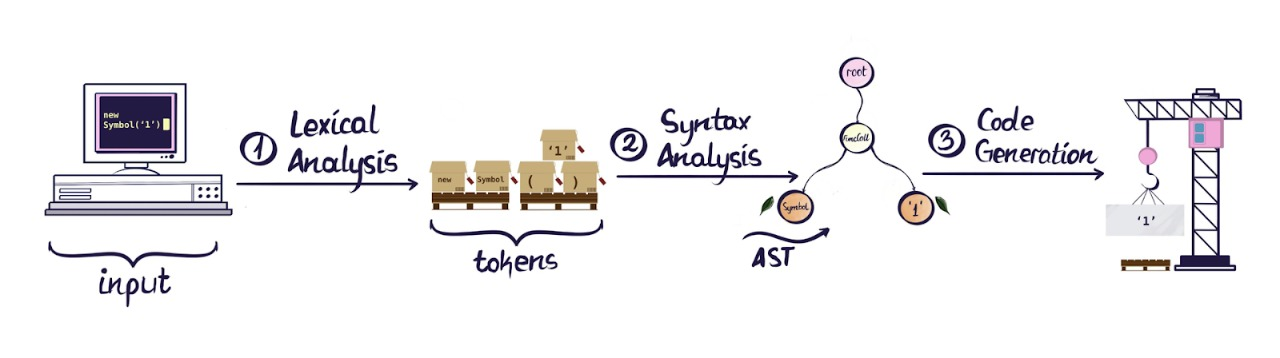
\includegraphics[width=230pt]{ast.jpeg}}
        \caption{ Transformation of a code by a compiler \cite{kundel_2020}. \\}
        \label{fig}
    \end{figure}


\vspace{15pt}

\section{Solution Outline}

\subsection{Deliverables}
\begin{itemize}
    \item A \href{https://github.com/vijay-jaisankar/aster}{Github Repository} containing the source code of Abstract syntax tree generator for the C language in C++.
    \item Project Report explaining the project and its working in detail. 
    \item README file containing the instructions on how to run the project.
    \item A Video Demo explaining the code and main features of the project.
\end{itemize}


\subsection{Work Split}
\begin{itemize}
    \item Mani Nandadeep -  Lexer and Grammar implementation
    \item R Prasanna - Parser, AST, and Grammar \\ implementation 
    \item Vijay Jaisankar - Parser, AST, and Grammar implementation
    \item M Dhanush - Lexer implementation, Parser
\end{itemize}


\subsection{References}
\begin{itemize}
    \item \textbf{Language Implementation Patterns} \cite{10.5555/1823613}: This book explains how existing language applications work and how certain concepts are implemented.
    \item  \textbf{Compilers: Principles and Practice } \cite{Compilers}: This book explains the phases and implementation of compilers and interpreters, using a large number of real-life examples. We will be using this book to understand the various stages of compiling and interpretting, as well as use it as a reference book for getting test cases and examples.
    \item \textbf{GNU Bison} \cite{GNUBison}:  Yacc-compatible parser generator. Bison is a general purpose parser generator that converts a grammar description for an LALR(1) context-free grammar into a C program to parse that grammar. We will be using Bison as a tool for inspiration; we can validate our outputs based on this tool, and see  how we can model our outputs based off of it.
    \item \textbf{Lex and YACC} \cite{LexYacc}: Lex helps write programs whose control flow is directed by instances of regular expressions in the input stream, i.e, Split the source file into tokens. Yacc provides a general tool for describing the input to a computer program. The Yacc user specifies the structures of his input, together with code to be invoked as each such structure is recognized. Yacc turns such a specification into a subroutine that handles the input process; frequently, it is convenient and appropriate to have most of the flow of control in the user's application handled by this subroutine,i.e, Find the hierarchical structure of the program. 
    \item \textbf{ AST Explorer} \cite{ASTExplorer}: We will use this tool to analyse visualisations of parse trees.


\end{itemize}

\vspace{15pt}


\bibliographystyle{ieeetr} % We choose the "plain" reference style
\bibliography{references} % Entries are in the refs.bib file




% * https://norasandler.com/2017/11/29/Write-a-Compiler.html
% * http://scheme2006.cs.uchicago.edu/11-ghuloum.pdf
% * https://ruslanspivak.com/lsbasi-part7/
% * https://www.101computing.net/abstract-syntax-tree-generator/
% * https://www3.nd.edu/~dthain/compilerbook/chapter6.pdf
% * https://github.com/jonatas/fast
% * http://icps.u-strasbg.fr/~pop/gcc-ast.html
% * https://github.com/afarah1/compiladores-ufrgs-2020-01
% * https://github.com/bamless/jstar
% * https://github.com/rmccullagh/compiler
% * https://www.cs.mcgill.ca/~cs520/2012/slides/ast.pdf
% * https://github.com/Yuhao-Lan/Compiler
% * https://github.com/gabrielzborges/AbstractSyntaxTree-C-Minus
% * https://github.com/buxlabs/abstract-syntax-tree
% * https://github.com/eliben/pycparser
% * https://www.cs.umd.edu/class/spring2017/cmsc430/slides/03-lexing-parsing.pdf
% * https://github.com/dvshapkin/mython



% !! IMPORTANT LINKS
% * https://github.com/connergdavis/simple-c-compiler
% * https://github.com/bbu/simple-interpreter
% * https://github.com/Tachone/Compiler/tree/master/grammar/%E8%AF%AD%E6%B3%95
% * https://github.com/thy-chan/Chan-s-C-Compiler/blob/master/source/lexSynAnalysis/test.txt
% * https://github.com/descent/simple_compiler



\end{document}
